


\newcommand{\nop}[1]{}
\documentclass[twocolumn]{svjour3}

\usepackage{amsmath}
%\usepackage[belowskip=-6pt,aboveskip=0pt]{caption}
\usepackage[lined,linesnumbered,resetcount]{algorithm2e}
\usepackage{amssymb}
\setcounter{tocdepth}{3}
\usepackage{graphicx}
\usepackage{tablefootnote}
\usepackage{url}
  
\usepackage{caption}
\usepackage{mathtools}
\DeclarePairedDelimiter\floor{\lfloor}{\rfloor}
\usepackage{IEEEtrantools}










\hyphenation{op-tical net-works semi-conduc-tor}


\begin{document}



\title{Design and Implementation of an Analytical Framework for Interference Aware Job Scheduling on Apache Spark Platform}




\author{Kewen Wang \\
Mohammad Maifi Hasan Khan \\ Nhan Nguyen \\ Swapna Gokhale}


\institute{ \at
Department of Computer Science and Engineering\\University of Connecticut \\
%              Tel.: +123-45-678910\\
  %            Fax: +123-45-678910\\
              \email{kewen.wang@uconn.edu, maifi.khan@uconn.edu,nhan.q.nguyen@uconn.edu,\\ssg@uconn.edu}           %  \\
%             \emph{Present address:} of F. Author  %  if needed
%           \and
   %        S. Author \at
      %        second address
}






%\date{Received: date / Accepted: date}




% make the title area
\maketitle

% As a general rule, do not put math, special symbols or citations
% in the abstract
\begin{abstract}

Apache Spark is one of the recently popularized open-source platforms that is increasingly being used for large-scale data analytic applications. However, while performance prediction in such systems is important for efficient job scheduling and optimizing resource allocation, interference among multiple Apache Spark jobs running concurrently in a virtualized environment makes it extremely difficult, which is addressed in this paper. Towards that, first, we develop data-driven analytical models to estimate the effect of interference among multiple Apache Spark jobs on job execution time in virtualized cloud environments. Next, we present the design of an interference aware job scheduling algorithm leveraging the developed analytical framework. We evaluated the accuracy of our models using four real-life applications (e.g., Page rank, K-means, Logistic regression, and Word count) on a 6 node cluster while running up to four jobs concurrently. Our experimental results show that the scheduling algorithm reduces the average execution time of individual jobs and the total execution time significantly, and ranges between 47\% to 26\% for individual jobs and 2\% to 13\% for total execution time respectively.\footnote{This paper is a significantly extended version of the authors' prior work~\cite{wangperformance,kewencloud} and includes the design and evaluation of interference aware job scheduling algorithms, which is not presented in prior efforts.}




\nop{
To maximize resource utilization and system throughput, hardware resources are often shared across multiple Apache Spark jobs through virtualization techniques in cloud platforms. However, while the performance of these jobs running in virtualized environment can be negatively affected due to interference caused by resource contention, it is nontrivial to predict the effect of interference on job performance in such settings, which is critical for efficient scheduling of such jobs and performance troubleshooting. To address this challenge, in this paper, first, we develop analytical models to estimate the effect of interference among multiple Apache Spark jobs running concurrently on job execution time in virtualized cloud environment. Second and finally, we present the design of an interference aware job scheduling algorithm leveraging the analytical framework for Apache Spark platform. We evaluated the accuracy of our models using four real-life applications (e.g., Page rank, K-means, Logistic regression, and Word count) on a 6 node cluster while running up to four jobs concurrently. Our experimental results show that the model can achieve high prediction accuracy, and ranges between 86\% to 99\% when the number of concurrent jobs are four and all start simultaneously, and ranges between 71\% to 99\% when the number of concurrent jobs are four and start at different times. Furthermore, the scheduling algorithm reduces the average execution time of individual jobs and the total execution time (i.e., completion time of the last job minus the start time of the first job) significantly, and ranges between 47\% to 26\% for individual jobs and 2\% to 13\% for total execution time respectively.\footnote{This paper is a significantly extended version of the authors' prior work~\cite{wangperformance,kewencloud} and includes the design and evaluation of interference aware job scheduling algorithms, which is not presented in prior efforts.} 
}


 



\end{abstract}

\keywords{Apache Spark \and Job Scheduling \and Performance Interference Modeling \and Execution Time Prediction}





\section{Introduction}
\noindent
Among many cloud computing platforms, Apache Spark~\cite{spark} is one of the popular open-source cloud platforms that introduces the concept of resilient distributed datasets (RDDs)~\cite{rdd} to enable fast processing of large volume of data leveraging distributed memory. Its in-memory data operations makes it well-suited for iterative applications such as iterative machine learning and graph algorithms. However, execution time of a particular job on Apache Spark platform can vary significantly depending on the input data type and size, design and implementation of the algorithm, and computing capability (e.g., number of nodes, CPU speed, memory size), making it extremely difficult to predict job performance, which is often needed to optimize resource allocation\cite{cloudopt}\cite{cloudscale}. Performance prediction can also help to locate execution stages with abnormal resource usage pattern~\cite{prepare}. 
While prior work exists that looked into the problem of performance prediction for cloud platforms such as Apache Hadoop \cite{hadoop} (an open-source implementation of MapReduce \cite{mr} computing framework), these approaches are not suitable for apache Spark platform due to its different programming model and features such as in-memory data operations.
\noindent
Hence, to address this void, in this paper, we focus on performance modeling for Apache Spark jobs. While various forms of machine learning approaches are often used to predict system performance leveraging past system execution data~\cite{stat}\cite{predict}\cite{oltp} and can achieve reasonable prediction accuracy, it requires training dataset. In contrast, modeling based approaches predict performance through modeling system behavior~\cite{starfish}\cite{nosqlmodel}\cite{pmodel}, and often can provide a better understanding regarding internal execution of a program and resulting performance. Therefore, in this paper, we apply analytical approaches to predict the performance of Apache Spark jobs. Specifically, we leverage the multi-stage execution structure of Apache Spark jobs to develop hierarchical models that can effectively capture the execution behavior of different execution stages. Using these models, we first measure the job performance based on limited scale execution using only a fraction of real data set. Next, we predict the job performance based on the limited scale execution job performance data. We evaluated our framework with four real-world applications. In each case, our model is able to predict execution time for individual stage with high accuracy. Additionally, the model is able to predict memory requirement for RDD creation with high accuracy. However, the accuracy of I/O cost prediction varied for different applications and simulation setup. We discuss our detailed findings in Section~\ref{evaluation}.

\noindent
The rest of the paper is organized as follows. Prior efforts that are related to our work is discussed in Section~\ref{related}. Section~\ref{overview} explains the models that are used to predict job performance in this work. Experimental results are presented in Section~\ref{evaluation}. Finally, Section~\ref{conclusion} concludes the paper.


\section{Related Work}
\label{related}
\noindent
With the proliferation of cloud computing platforms, significant volume of prior work looked into the problem of performance modeling in cloud settings and distributed systems in general~\cite{predict,nosqlmodel,pmodel,starfish,oltp,prepare,cloudopt,cloudscale,dbseer,amml}. 
Among these, PREDIcT~\cite{predict} looks into the problem of predicting runtime for network intensive iterative algorithms and focuses on Hadoop MapReduce platform. Starfish~\cite{starfish} leverages analytical approaches to predict job performance based on job simulation data. CloudScope \cite{chen2015cloudscope} is one of the more recent efforts that employs a discrete-time Markov Chain model to predict the performance interference of co-resident applications by modeling an application as a sequence of job slices and estimating the probability of a job moving from one state to another considering different factors such as current workloads and slowdown. Matrix~\cite{chiang2014matrix} utilizes machine learning methods to predict application performance on virtual machines by applying clustering methods to classify applications and predicts the performance of new applications by comparing against the previously trained models. 


\noindent
Interference modeling among multiple applications running on MapReduce framework is tried before as well for the purpose of efficient job scheduling~\cite{bu2013interference} that requires training using different combinations of applications, which can quickly become prohibitive. MIMP~\cite{zhangmimp} presents a progress aware scheduler for Hadoop framework that applies regression model to train and predict task completion time based on past execution. HybridMR \cite{sharma2013hybridmr} presents another MapReduce scheduler for hybrid data center consisting of physical and virtual machines. This scheduler uses performance interference models to guide resource allocation, and applies linear and non-linear exponential regression model to capture CPU, I/O, and memory interference. 


\noindent
While these prior efforts provide invaluable insight to the problem of performance modeling, however, most of them use black-box approaches and can not be extended easily without retraining. Moreover, due to the multi-stage execution model and in-memory computation feature of Apache Spark platform, it is non-trivial to apply these approaches without further modifications for predicting the effect of interference on job execution time. As such, we focus on developing data-driven analytical models for modeling interference among multiple Apache Spark jobs which is complementary to prior efforts. 



\section{Overview}
\label{overview}

\noindent
Each Apache Spark job typically consists of multiple execution stages where each stage implements certain operations and is executed sequentially. Moreover, to facilitate parallel processing, input data set is partitioned into multiple sets and are distributed over multiple worker nodes. Within each worker node, multiple batches of tasks are launched to process the corresponding partition of the input data. The number of tasks within each node is determined based on the size of the input data and configuration settings of the program. For example, if the input data size of the PageRank job is 2.5 GB, the total number of input blocks will be 40 for a default block size of 64 MB. As the number of tasks is equal to the number of input blocks and the number of tasks in each stage is same within one Spark job, there will be 40 tasks in each stage. However, different CPU core may complete different number of tasks due to the differences in computing ability and uncertainty during the program execution. \nop{
\begin{figure}[!t]
\centering
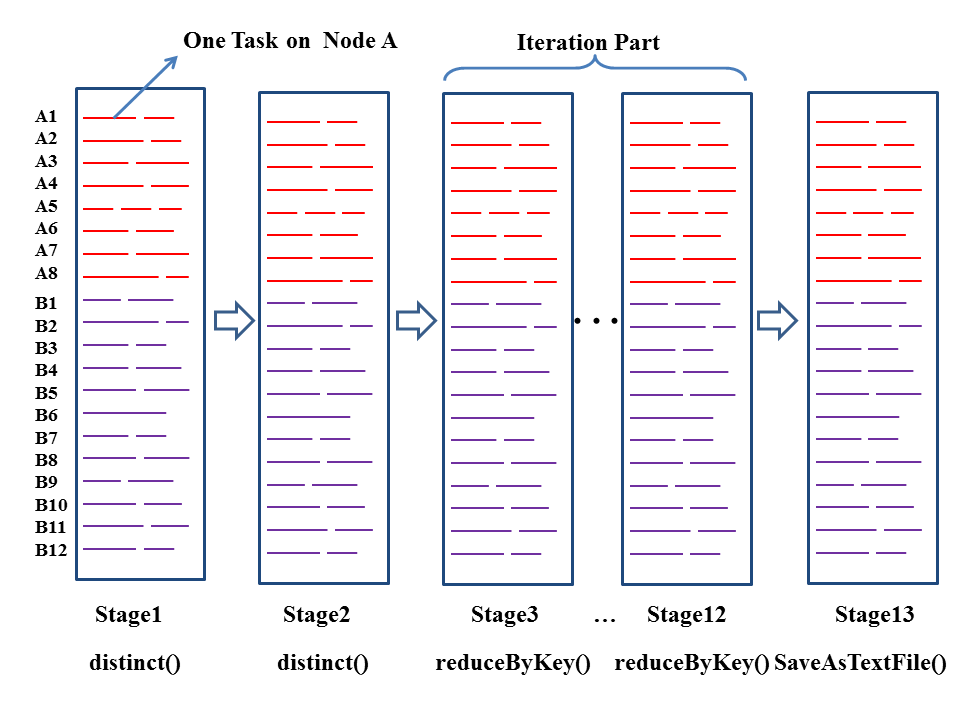
\includegraphics[width=3.0in]{flow.png}
\caption{Prediction Accuracy for WordCount}
\label{flow}
\end{figure}
}
\begin{figure}[!t]
\centering
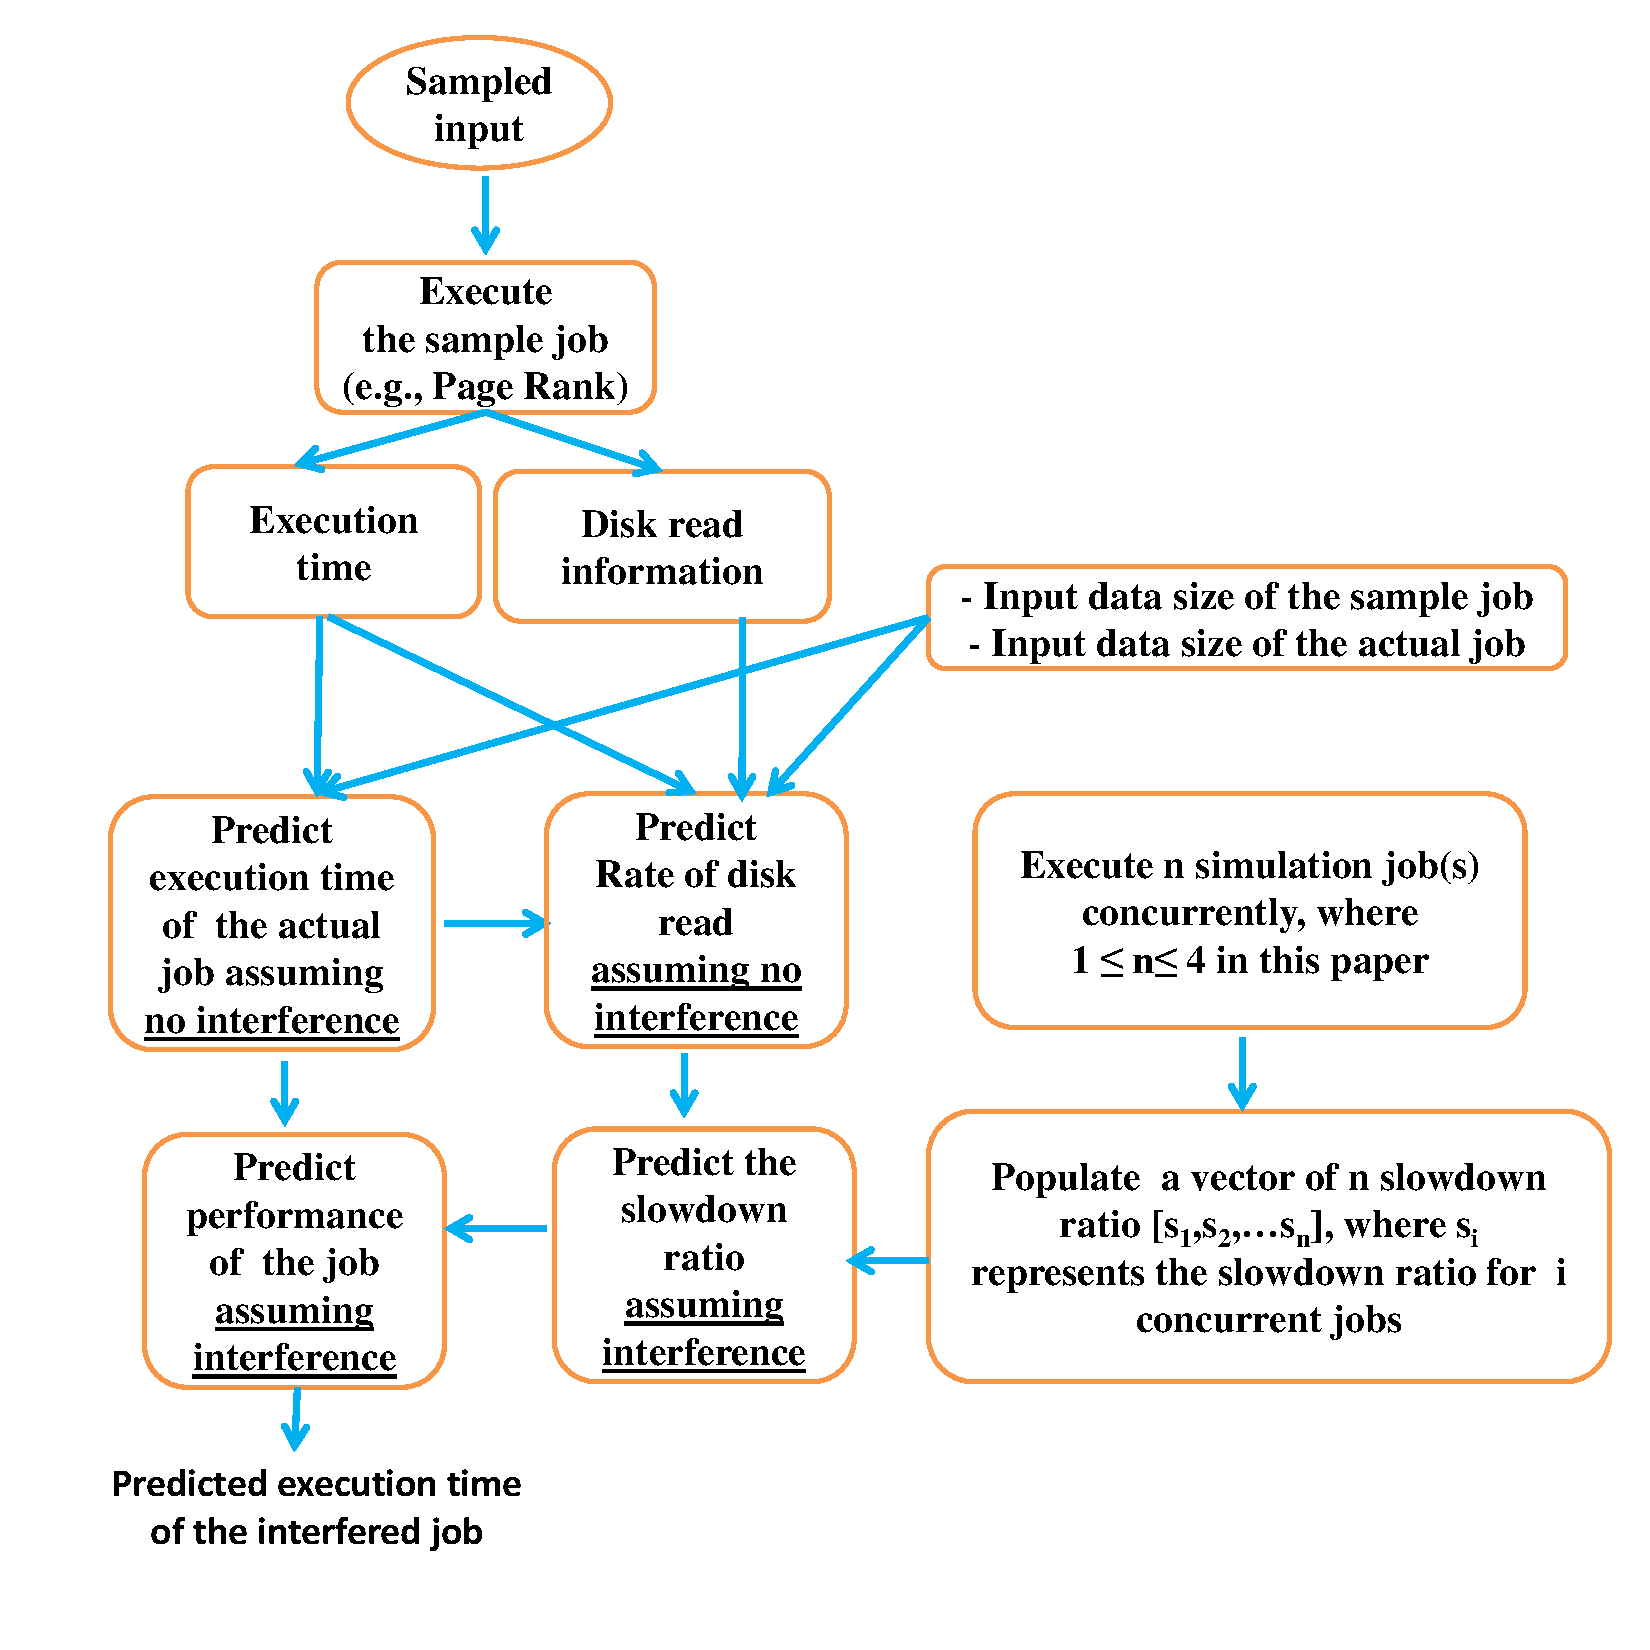
\includegraphics[width=3.3in]{flow1.pdf}
\caption{Performance Prediction for Interfered Jobs}
\label{flow}
\end{figure}

\noindent
Given the above multistage execution model, the main idea behind our work is as follows (Figure~\ref{flow}). First, for a given Apache Spark job, we predict the execution time for each stage leveraging the performance model developed based on the performance of the actual job with smaller input data set. Note that this model is presented in our prior work~\cite{wangperformance}, and assumes that there are no interference in the system from other jobs. Next, we estimate the slowdown ratio for a given number of jobs running concurrently by executing our simulation job, which is implemented by us (more details in Section~\ref{evaluation}) and is different than any of the four jobs that we used for evaluation. However, as the slowdown ratio due to interference among simulated jobs can be different compared to the actual jobs, for a given job, we adjust the expected slowdown ratio by taking into account the actual job parameters such as input data size and disk I/O characteristics. Once we estimate the expected slowdown ratio, we estimate the execution time considering the interference. For completeness, we first briefly present the model that is used to predict execution time assuming no interference from our earlier work~\cite{wangperformance}, and then present the model for predicting the slowdown ratio due to interference that allows us to predict the execution time in the presence of interference among multiple jobs. 


\subsection{Model for Estimating Execution Time}
\label{oldmodel}
As an Apache Spark job is executed in multiple stages where each stage contains multiple tasks, we use the following notation to represent an Apache Spark job.
\begin{IEEEeqnarray}{rCl}
\label{jobperform}
Job &{} ={}& \{Stage_i \mid 0 \leq i \leq M \} \\
Stage_i &{} ={}& \{Task_{i,j} \mid 0 \leq j \leq N \} 
\end{IEEEeqnarray}

\noindent
Here $M$ is the number of stages in a job and $N$ is the number of tasks in a stage. 

\noindent
Next, as different stages within a job are executed sequentially, we represent the execution time of a job as the sum of the execution time of each stage plus the job startup time and the job cleanup time as follows.
\begin{IEEEeqnarray}{rCl}
\label{jobtime}
\hspace{-0.4cm}
JobTime = Startup + \sum_{s=1}^{M}StageTime_{s} + Cleanup
\end{IEEEeqnarray}
Next, within each stage, as one CPU core executes one task at a time, in a cluster with $H$ worker nodes, the number of tasks $P$ that can run in parallel is calculated as follows.

\begin{IEEEeqnarray}{rCl}
\label{paralltask}
P=\sum_{h=1}^H CoreNum_{h}
\end{IEEEeqnarray}

\noindent
Here $CoreNum_{h}$ is the number of CPU cores of working node $h$ and $H$ is the number of working nodes in the cluster. Hence, within an execution stage, tasks in each stage are executed in batches where each batch consists of $P$ tasks running in parallel. However, due to the differences in computing capabilities among different worker nodes in a cluster and inherent uncertainty in program execution, the execution time of different tasks may vary significantly. Therefore, the time spent in a particular stage can be calculated as the maximum of the sum of all the sequential tasks' time within a stage plus the stage startup time and the stage cleanup time as follows.

\begin{IEEEeqnarray}{rCl}
\label{stagetime}
StageTime&{} ={}& Startup + \max_{c=1}^{P} \sum_{i=1}^{K_c} TaskTime_{c,i} \nonumber \\
&&+Cleanup
\end{IEEEeqnarray}

\noindent
Here $P$ is the number of total CPU cores, and $K_c$ is the number of sequential tasks executed on CPU core $c$.

\noindent
Finally, as different tasks in a stage follow the same execution pattern, the execution time of a task can be computed as follows.

\begin{IEEEeqnarray}{rCl}
\label{tasktime}
TaskTime&{} ={}& DeserializationTime + RunTime \nonumber \\
&&+ SerializationTime
\end{IEEEeqnarray}

\noindent
Here $DeserializationTime$ is the time taken to deserialize the input data, $SerializationTime$ is the time taken to serialize the result, and $RunTime$ is the actual time spent performing operations on data such as data mapping, filtering, calculation, and analyses. 
Based on the above model, to predict job performance, the presented framework first executes the program on a cluster using limited amount of sample input data and collects performance metrics such as run time during the simulated run. 

\noindent
Next, to predict the execution time of the actual run based on the extracted performance metric from simulated run, we first calculate the number of tasks $N$ where $ N = InputSize / BlockSize $, $InputSize$ is the size of the input data, and $Blocksize$ is the size of one data block in HDFS. 
The tasks within a stage are scheduled to run batch by batch, and the number of tasks $P$ in each batch is computed as shown in equation (\ref{paralltask}). In one batch of tasks, while the tasks may start simultaneously, they may not finish at the same time due to various factors such as data skew problem, and differences in computing capability of different worker nodes. Hence, using sampled data, we calculate the average execution time for a task for a given stage for a worker node $h$ as follows. 
\begin{IEEEeqnarray}{rCl}
\label{taskest}
TaskRunTime_{h,i} &{} ={}& DeserializeTime_{h,i} \nonumber \\
&&+ RunTime_{h,i} \nonumber \\
&&+ SerializationTime_{h,i} \\
\label{avgtask}
AvgTaskTime_h &{} ={}& \frac{1}{n_h}\sum_{i=1}^{n_h} TaskRunTime_{h,i}
\end{IEEEeqnarray}
Here $n_h$ is the number of tasks running in host $h$ in a particular stage of the sample job. 
Moreover, during our experiment, we observed that the average execution time of the first batch is significantly different compared to the subsequent batches within the same stage, which we capture as follows. 
\begin{IEEEeqnarray}{rCl}
\label{ratio}
Ratio_h=\frac{\frac{1}{n_h-P_h} \sum_{i= P_h + 1}^{n_h}TaskTime_{h,i}}{\frac{1}{P_h} \sum_{j=1}^{P_h} TaskTime_{h,j}}
\end{IEEEeqnarray}
Here $n_h$ is the number of tasks running in host $h$, and $P_h$ is the number of tasks in the first batch. As tasks execute on different hosts in parallel, to predict the execution time for a particular stage during actual execution, stage $Startup$ time and $Cleanup$ time are viewed as constants which are extracted from simulation logs, and stage execution time is estimated as follows.
 
\begin{IEEEeqnarray}{rCl}
\label{stageest}
EstStageTime&{} ={}&Startup + \max_{c=1}^{P} \sum_{i=1}^{K_c} AvgTaskTime_{c,i} \nonumber \\
&& +  Cleanup \\ 
\nonumber \\
\label{stagetask}
EstTaskTime_{c,i}&{} ={}&\left\{\begin{IEEEeqnarraybox}[\relax][c]{l's}
AvgTaskTime_c,& $i = 1$\\
AvgLaterTaskTime_c,& $i > 1$%
\end{IEEEeqnarraybox}\right.
\end{IEEEeqnarray}



\noindent
Here $P$ is the number of total CPU cores calculated in equation (\ref{paralltask}) and $K_c$ is the number of sequential tasks running on CPU core $c$. $AvgTaskTime_c$ is the average time of the tasks of the first batch running on CPU core $c$ for the corresponding host, which is calculated in equation (\ref{avgtask}). $AvgLaterTaskTime_c$ is the average time of the tasks of the following batches, which is calculated as $Ratio_h \times AvgTaskTime_h$.

\noindent
While we can apply the prediction model presented in this section to estimate the execution time for a single job assuming no interference~\cite{wangperformance}, we still need a way to predict the slowdown ratio when interfered with other jobs, which we address as follows.


\subsection{Modeling Interference}
As different stages of a job is expected to have different characteristics in terms of resource utilization (e.g., CPU, I/O, memory), different stages of multiple jobs running concurrently on a system is expected to result in different interference patterns, affecting the execution time differently. Based on this observation, we model the slowdown ratio due to interference among multiple jobs for each stage separately. Towards that, in our model, each stage is represented as a vector consisting of execution time, CPU usage, disk I/O rate, and network I/O rate as follows.
\begin{equation}
\label{res}
Res_i = (RunTime_i, CPU_i, DiskIO_i, NetIO_i)
\end{equation}
Here $1 \leq i \leq M$, and $M$ is the number of stages in a job. Memory was not one of the bottleneck resources in our case. As such, we only considered Disk I/O and did not consider memory utilization in our model, which can be incorporated if needed for certain platforms/scenarios. 





\par \noindent 
Next, the slowdown resulting from interference with other applications for a particular stage is represented as follows.
\begin{equation}
\label{slowdownratio}
SlowdownRatio(Stage_{i,k})
= f(Res_{i,k},Res_{Other jobs})
\end{equation}
\nop{
\begin{equation}
\label{setS}
SetS = \{Stage_{k,i} \mid 1 \leq k \leq J \ , 1 \leq i \leq M \}
\end{equation}
}
\noindent
Here $1 \leq k \leq J$, $1 \leq i \leq M$, $J$ is the number of jobs running in parallel, and $M$ is the number of stages in the Apache Spark job. $Res_{Otherjobs}$ represents the resources consumed by other jobs that are running concurrently with $Stage_{i,k}$. 
Simply put, this slowdown ratio is the ratio between execution time with interference over execution time without interference for a particular stage. Hence, once we estimate the value of the slowdown ratio and the expected execution time when there is no interference, we can estimate the execution time if there are interference with other jobs. 


%Please note that, once we collect the resource usage profile by running sample jobs, we need to estimate the execution time of original job. The difference between original job and sample job is the size of input data, which decides the number of tasks in one stage.
\noindent
As the slowdown happens primarily due to contention for bottleneck resources in the system, to better understand the underlying reasons behind the slowdown, we ran a series of experiments and collected job event logs and resource consumption data, and then extracted the resource usage profile for each stage. Job event log is generated by Apache Spark platform, and resource consumption data is collected using system monitoring tool dstat \cite{dstat}. Apache Spark log records the time line of different stages of a running job, which was used to determine the submission and completion time of different stages of a job. The resource usage for different stages of a job is represented as below: 
\begin{equation}
\label{cpu}
CPU_i 
= (CPUusr_i, CPUsys_i, CPUidle_i, CPUwait_i) 
\end{equation}
\begin{equation}
\label{diskio}
DiskIO_i = (RateofDiskRead_i, RateofDiskWrite_i)
\end{equation}
\begin{equation}
\label{netio}
NetIO_i = (RateofNetReceive_i, RateofNetSend_i)
\end{equation}
Here $1 \leq i \leq M$, and $M$ is the number of stages in a Apache Spark job.
\noindent 
As an Apache Spark job uses in-memory data processing to reduce execution time, in the first stage of a job, it reads the input data to memory, and then analyzes the in-memory data in the subsequent stages. Due to this characteristic, in the first stage, frequent I/O is expected, leading to longer I/O wait. Based on this observation, as bulk of the disk I/O happens in the first stage, in our model, we calculate the slowdown ratio for the first stage only, and assume that the slowdown ratio in cases where the first stage interferes with the following stages from another job is 1.0 (i.e., the slowdown due to interference is expected to be minimal). Note that, while this assumption is not accurate for certain jobs and stages, the error introduced due to this assumption in prediction accuracy is not significant in our case. 

\nop{
In our cluster, the Maximum network transaction speed is 118MB/s tested by using iperf command, and the maximum disk I/O is 266MB/s tested by using dd command. We find that the network I/O or disk I/O speed can not reach the maximum value when we run Apache Spark job in the cluster, but the cpu usage often achieves high value. From this observation, we infer that the bottleneck of Apache Spark job is often in CPU usage, which determines the execution time of the job stage. CPU usage is calculated as the sum of the user and system CPU usage. And high level of CPU usage means the high processing speed in this stage, which will result in less execution time.
}


\noindent 
As most of the time spent in the first stage is due to reading data from disk to memory, we represent the relationship between the amount of data read in the first stage (e.g., size of input data), the rate of disk read, and the execution time of the first stage as follows: 
\begin{equation}
\label{diskread}
RunTime_{Stage 1}=c \times \frac{Input Data Size}{Rate of DiskRead_{Stage 1}} \end{equation}
\noindent 
Now, if we assume that we execute the same job twice, once with the reduced input data set (i.e., sample job) and once with the complete input data set (i.e., complete job), from equation~\ref{diskread}, we can have the following. The word {\textit{Int.}} refers to {\textit{Interference}} in the following equations. 


\begin{eqnarray}
\label{sampleFull}
\begin{gathered}
\frac{InputDataSize_{Sample job}}{InputDataSize_{Complete job}} = \\
\frac{Rate of Disk Read_{Sample job, Stage 1}}{RateofDiskRead_{Complete job, Stage 1}} \times \\
\frac{RunTime_{Sample Job, Stage 1}}{RunTime_{Complete job without Int., Stage 1}}
\end{gathered}
\end{eqnarray}


Based on equation~\ref{sampleFull}, we can have the following equation for predicting the rate of disk read for a complete job. 


\begin{eqnarray}
\label{fullDiskIORead}
\begin{gathered}
Predicted Rate of Disk Read_{Complete Job without Int., Stage1}  = \\
Rate of Disk Read_{Sample Job, Stage 1} \times \\
\frac{RunTime_{Sample Job, Stage 1}}{RunTime_{Complete Job without Int., Stage 1}} \\
\times \frac{Input Size_{Complete Job}}{Input Size_{Sample Job}}
\end{gathered}
\end{eqnarray}

\noindent
In the above equation, we can estimate the value of $RunTime_{Complete Job without Int., Stage 1}$ using the model described in Section~\ref{oldmodel}~\cite{wangperformance}. Once we predict the rate of disk read for a complete job with no interference, next, we need to model the relation between the rate of disk read and the slowdown ratio when there is interference. For that, first, we run a simulation program (written by us as described in Section~\ref{evaluation}) to collect the runtime information with and without interference and calculate the parameter $\beta_{n}$ as follows.
\begin{equation}
\label{beta}
\begin{gathered}
\beta_{n} = \frac{1}{Rate of Disk Read_{Simulation Run without Int., Stage 1}} \times \\
(\frac{RunTime_{Simulation Run with Int. for n jobs, Stage 1}}{RunTime_{Simulation Run without Int., Stage 1}} - \\
\floor*{\frac{RunTime_{Simulation Run with Int. for n jobs, Stage 1}}{RunTime_{Simulation run without Int., Stage 1}}})
\end{gathered}
\end{equation}
\noindent
In this paper, we assume that there can be at most 4 concurrent jobs in a system, and varied $n$ between 2 to 4 to calculate $\beta_{2}$, $\beta_{3}$, and $\beta_{4}$. Running the simulation job and calculating $\beta_{n}$ take only few minutes and need to be done only once for a given environment. Next, we use $\beta_{n}$ to estimate the slowdown ratio when there are $n$ concurrent jobs in the system as follows.

\begin{equation}
\label{slowdisk}
\begin{gathered}
SlowdownRatio(Stage_{(1,k)})=\\
\frac{RunTime_{Complete Job with Int., Stage 1}}{RunTime_{Complete Job without Int., Stage 1}} = \beta_{n} \\
\times PredictedRateofDiskRead_{Complete Job without Int., Stage 1} \\ + \floor*{\frac{Run Time_{Simulation run with Int., Stage 1}}{Run Time_{Simulation Run without Int., Stage 1}}}
\end{gathered}
\end{equation}



\subsection{The Cascading Effect}
Given the above formulation, if we assume that all the jobs are of same type and start at the same time, modeling interference is straightforward as they all have the same execution behavior in each stage. However, for interference among different types of jobs possibly starting at different times, this is a bit more complicated due to the possible cascading effect. For example, the slowdown of stage 1 of job $A$ may push this stage to interfere with stage 2 of job $B$. Hence, a dynamic interference estimation algorithm is designed to solve this problem. The main idea behind the algorithm is as follows. First, the algorithm uses the execution time line of each job as input, and calculates the slowdown ratio for each stage of different jobs within the same time slot, and generates the execution time line of each job under interference condition. Based on that, the algorithm identifies the job that will finish its first stage the earliest, removes that job from the list, and recalculates the effect of interference for the remaining jobs for the remainder of the execution time. The algorithm applies this repeatedly until the list becomes empty. This dynamic interference estimation algorithm is described in Algorithm~\ref{algo} (Appendix).





\subsection{Interference Aware Job Scheduling}
\label{scheduler}

Finally, as concurrent Apache Spark jobs often heavily interfere, especially at the first stage, to minimize interference and job execution time, we design and implement a scheduler that automatically schedules and executes submitted Spark jobs leveraging the performance prediction framework presented earlier. Specifically, when a new job arrives in the system, if there is no existing job in the system, the scheduler locates available servers that can execute the job and starts the job immediately. However, if there are existing jobs running in the system with possibly more jobs waiting in the queue, the scheduler calculates the waiting time (if any) of the new job and readjusts the waiting time of the jobs that are already in the queue (if needed) to determine the best scheduling plan and updates the scheduling file accordingly (Note that jobs are not executed on first-come-first serve basis in our system). 

\noindent
The process of calculating the waiting time for a job in multiple steps is illustrated in Figure \ref{scheexample}. Here we assume that the first job $J_1$ is submitted at time point $T_1$, and is started immediately as there is no other job in the system. The second job $J_2$ is submitted at time $T_2$. At that time, the scheduling algorithm calculates the amount of time already executed by $J_1$ (i.e., $T_2-T_1$) to decide whether $J_2$ can be started immediately or needs to wait to avoid interference. If $J_2$ needs to wait, the algorithm calculates the tentative wait time for $J_2$ based on the interference model, which is $\Delta T$, and updates the scheduling file by writing the waiting period $\Delta T$ for $J_2$.

\noindent
Now, let us assume that, at time point $T_3$, the third job $J_3$ arrives in the system. At that point, the algorithm first calculates the execution time (which is different than the wall clock time) of the two jobs already running in the system. As $J_1$ executed alone before $S_1$ and executed concurrently with $J_2$ between $S_1$ and $T_3$, we calculate the execution time of $J_1$ since the last job submission time (i.e., $T_2$) as $ExeTime_{J1} = (S_1-T_2)+(T_3-S_1) \times Ratio_{J_1}$, and the execution time for $J_2$ as $ExeTime_2 = (T_3-S_1) \times Ratio_{J_2}$, where $Ratio_{J_1}$ and $Ratio_{J_2}$ are the slow down ratio of $J_1$ and $J_2$ respectively when interfered with one job. Note that the slowdown ratios are different for different jobs due to differences in job characteristics. Also, as the job profiles in the scheduling file are updated every time a new job is submitted, we only need to estimate the execution time for each running job since the last job submission time. 

\noindent
After calculating the execution times for these two jobs (which tell us what stage each job is at currently), we update the job profiles for $J_1$ and $J_2$, and then decide whether $J_3$ can start immediately or not, based on the possibility of interference with the currently running jobs. 

\noindent
While calculating the execution time, we have to consider the possibility that each job may interfere with different jobs at different points in time during the execution. To handle this possibility, the algorithm saves the start and end time point of the first stage for each job (as the significant interference happens in the first stage of a job), and sorts the list based on start time points, and determines which set of jobs interfere at a particular point in time, and calculates the execution time incrementally. 

\begin{figure}[!t]
\centering
\captionsetup{justification=centering}
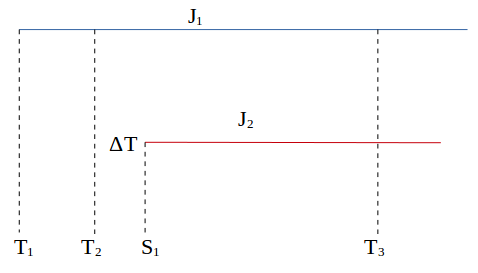
\includegraphics[width=3in]{ScheExample.png}
\caption{A Scheduling Example}
\label{scheexample}
\end{figure}




\noindent




\noindent
The algorithm to determine the waiting time for a job is shown in Algorithm~\ref{algoschedule} (Appendix) which has two main parts. The first part of the algorithm consists of the function depicted in Algorithm~\ref{algoexe} (Appendix) that calculates the execution time of the previously submitted jobs and updates the job schedule file (Algorithm~\ref{algoupdate} (Appendix)). The second part consists of Algorithm~\ref{algofind}(Appendix) that searches the combination of waiting times and job schedules that will minimize the total execution time. 












\begin{figure}[!t]
\centering
\captionsetup{justification=centering}
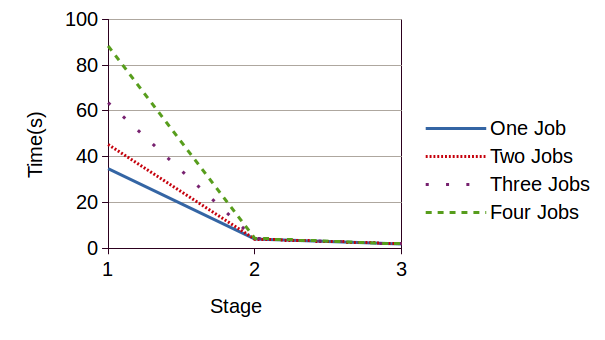
\includegraphics[width=3in]{simjobs.png}
\caption{Execution Time for Different Number of Simulation Jobs}
\label{simjobs}
\end{figure}

\begin{table*}[!htb]
\renewcommand{\arraystretch}{1.3}
\caption{Prediction Accuracy for Interference Among Same Jobs}
\label{table_samejob}
\centering
\begin{tabular}{c|c|c|c}
\hline
\bfseries JobName & \bfseries Job Number & \bfseries First Stage & \bfseries Whole Job\\
\hline\hline
PR & 2 & 0.97 & 0.80\\
& 3 & 0.96 & 0.85\\
& 4 & 0.92 & 0.82\\
\hline
KM & 2 & 0.75 & 0.70\\
& 3 & 0.71 & 0.68\\
& 4 & 0.98 & 0.92\\
\hline
LR & 2 & 0.74 & 0.78\\
& 3 & 0.79 & 0.81\\
& 4 & 0.97 & 0.97 \\
\hline
WC & 2 & 0.87 & 0.86\\
& 3 & 0.96 & 0.94\\
& 4 & 0.95 & 0.94\\
\hline
\end{tabular}
\end{table*}


\begin{table*}[!htb]
\renewcommand{\arraystretch}{1.3}
\caption{Execution Time Prediction for Four Interfered PageRank Jobs}
\label{pr20gprIII}
\centering
\begin{tabular}{l|r|r|r|r|r|r}
\hline
\bfseries StageNo & \bfseries 1 & \bfseries 2 & \bfseries 3 & \bfseries 4 & \bfseries 5 & \bfseries 6 \\
\hline \hline
Actual Time (s)
& 652.7
& 37.3 
& 32.3 
& 23.9 
& 23.2
& 58.8 \\
\hline
Predicted Time (s) 
& 594.3 
& 43.0 
& 10.6
& 5.4 
& 5.0 
& 28.3 \\
\hline
\end{tabular}
\end{table*}

\begin{table*}[!htb]
\renewcommand{\arraystretch}{1.3}
\caption{Execution Time Prediction for Four Interfered K-Means Jobs}
\label{km20gkmIII}
\centering
\begin{tabular}{l|r|r|r|r|r|r|r|r|r|r|r|r}
\hline
\bfseries StageNo & \bfseries 1 & \bfseries 2 & \bfseries 3 & \bfseries 4 & \bfseries 5 & \bfseries 6 & \bfseries 7 & \bfseries 8 & \bfseries 9 & \bfseries 10 & \bfseries 11 & \bfseries 12\\
\hline \hline
Actual Time (s)
& 688.4
& 7.1
& 19.9
& 8.1
& 16.5
& 7.4
& 15.9
& 7.2
& 15.8
& 7.0
& 15.6
& 7.0 \\
\hline
Predicted Time (s) 
& 708.3
& 7.4
& 25.2
& 18.1
& 22.9
& 9.7
& 23.6
& 8.4
& 23.2
& 9.2
& 24.8
& 6.2 \\
\hline
\end{tabular}
\end{table*}

\begin{table*}[!htb]
\renewcommand{\arraystretch}{1.3}
\caption{Execution Time Prediction for Four Interfered Logistic Regression Jobs}
\label{lr20glrIII}
\centering
\begin{tabular}{l|r|r|r|r|r|r|r|r|r|r}
\hline
\bfseries StageNo & \bfseries 1 & \bfseries 2 & \bfseries 3 & \bfseries 4 & \bfseries 5 & \bfseries 6 & \bfseries 7 & \bfseries 8 & \bfseries 9 & \bfseries 10 \\
\hline \hline
Actual Time (s)
& 649.6
& 7.3
& 7.5
& 7.3
& 7.4
& 7.2
& 7.5
& 7.2
& 7.5
& 7.4\\
\hline
Predicted Time (s) 
& 669.2
& 7.1
& 7.2
& 7.6
& 6.6
& 7.0
& 6.5
& 7.9
& 6.9
& 6.3 \\
\hline
\end{tabular}
\end{table*}


\begin{table*}[!htb]
\renewcommand{\arraystretch}{1.3}
\caption{Execution Time Prediction for Four Interfered WordCount Jobs}
\label{wc20gwcIII}
\centering
\begin{tabular}{l|r|r}
\hline
\bfseries StageNo & \bfseries 1 & \bfseries 2 \\
\hline \hline
Actual Time (s)
& 598.8
& 66.8 \\
\hline
Predicted Time (s) 
& 631.8
& 77.8 \\
\hline
\end{tabular}
\end{table*}


\nop{maifi
\begin{figure}[!htb]
\centering
\captionsetup{justification=centering}
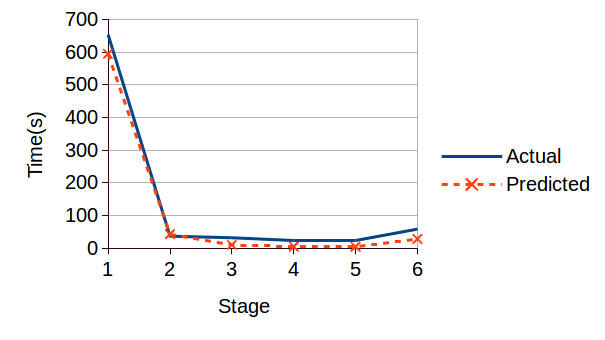
\includegraphics[width=3in]{pr20g_prIII.png}
\caption{Execution Time Prediction for Four Interfered PageRank Jobs}
\label{pr20gprIII}
\end{figure}
\begin{figure}[!t]
\centering
\captionsetup{justification=centering}
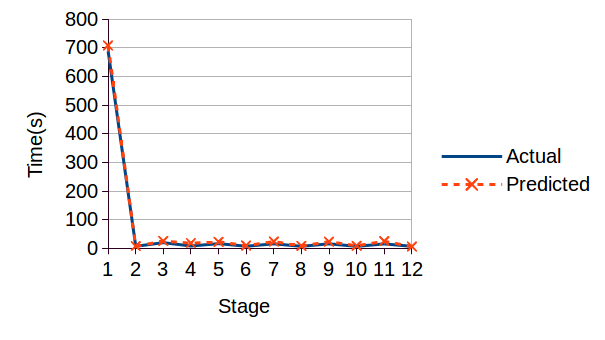
\includegraphics[width=3in]{km20g_kmIII.png}
\caption{Execution Time Prediction for Four Interfered K-Means Jobs}
\label{km20gkmIII}
\end{figure}


\begin{figure}[!htb]
\centering
\captionsetup{justification=centering}
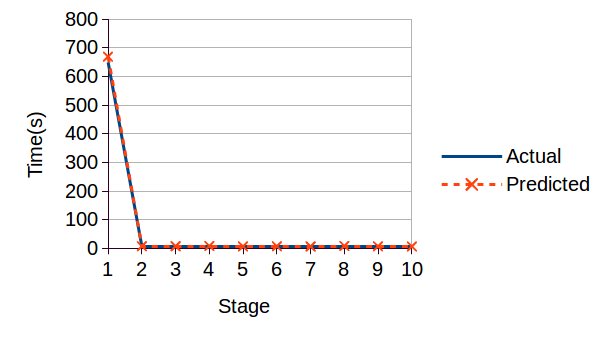
\includegraphics[width=3in]{lr20g_lrIII.png}
\caption{Execution Time Prediction for Four Interfered Logistic Regression Jobs}
\label{lr20glrIII}
\end{figure}
\begin{figure}[!t]
\centering
\captionsetup{justification=centering}
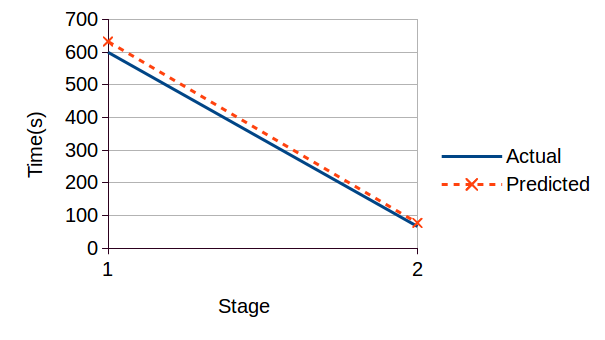
\includegraphics[width=3in]{wc20g_wcIII.png}
\caption{Execution Time Prediction for Four Interfered WordCount Jobs}
\label{wc20gwcIII}
\end{figure}
}







\section{Evaluation}
\label{evaluation}

\noindent
To evaluate the accuracy of our modeling framework and the performance of the job scheduling algorithm, we used a cluster of 6 machines. Each machine had 8 CPU cores (Intel(R) Xeon(R) CPU E5620, 2.40GHz) and 22 GB of RAM memory where each machine hosted 4 virtual machines. We used Xen hypervisor \cite{xen} to create up to four virtual machines on each physical machine. Each virtual machine was configured with 4GB of RAM memory and 1 CPU core. For the deployed Apache Spark platform, one machine served as the master node, and the remaining five machines served as the working nodes. We created multiple clusters leveraging virtual machines to execute multiple Apache Spark jobs in parallel. 


\noindent
In our evaluation, for prediction, first, we need to estimate the parameter $\beta_{n}$ in equation (\ref{beta}). Towards that, we implemented our own Apache Spark job and executed that on our cluster to obtain the execution time and resource consumption information. This simulation job consists of three stages executing distinct(), groupByKey(), and count() operation respectively. Distinct() implements a mapping function and parses the input data, groupByKey() processes the output of distinct() operation, and count() is a CPU intensive operation performing data summarization. This simulation job is executed with 2.5 GB of sample data where the first stage implementing the Distinct() operation involves significant I/O compared to the following two stages. To measure $\beta_{n}$, we executed $n$ ($n$=1,2,3,4) instances of this simulation job in parallel. As shown in Figure \ref{simjobs}, the effect of interference is significant for the first stage but minimal for the subsequent stages. 





\noindent
Once we estimated the value of $\beta_{n}$, subsequently, we used our formulation to predict the execution time for each stage of each job separately considering different execution scenarios and added up the prediction error for each stage to calculate the total prediction accuracy $R$ as below.
\begin{equation}
\label{predictaccuracy}
R = |1 -  \frac{\sum_{i=1}^{M}|PredictedTime_i - MeasuredTime_i|}{\sum_{j=1}^{M} MeasuredTime_{j}}|
\end{equation}
\noindent
Here $M$ is the number of stages in a job, $PredictedTime_i$ is the predicted execution time for $stage_i$, and \\
$MeasuredTime_i$ is the actual execution time of $stage_i$. Different evaluation scenarios are presented below.

\subsection{Interference Among Multiple Jobs of the Same Type Starting Simultaneously}

\noindent
In a shared cluster, multiple Apache Spark jobs running on separate virtual machines hosted on the same physical machine can cause significant interference, impacting the performance of each job. However, as different jobs may have different execution patterns and resource requirements, estimating the effect of interference on performance is nontrivial. As such, to demonstrate the generalizability of our work, we validated our model using four different Apache Spark jobs, namely, PageRank, K-Means, Logistic Regression and WordCount. The jobs vary in terms of the number of stages, the number of tasks, and the library functions they use to implement the job. For example, WordCount counts the word frequency for a given text file. K-Means implements a clustering algorithm, and Logistic Regression implements the Logistic Regression algorithm, which are examples of machine learning jobs. Finally, PageRank is an example of graph analyzing and processing jobs. For testing, we used the LiveJournal network dataset from SNAP \cite{snap} for PageRank, which is processed through mapping each node id onto a longer string to form a 20 GB input data set. K-Means and Logistic Regression used 20 GB of numerical Color-Magnitude Diagram data of galaxy from Sloan Digital Sky Survey (SDSS) \cite{sdss}. WordCount application used 20 GB of Wikipedia dump data.


\noindent
In this part of the evaluation, we present the accuracy of prediction while modeling the effect of interference among multiple jobs of the same type (e.g., interference between n instances of job x).





\noindent

For prediction, we first executed the sample job (e.g., Page rank) with 2.5 GB of input data which was extracted from the actual input data to collect the job execution profile. We ensured that no other job was running during this execution. The collected execution trace was then used to predict the execution time assuming no interference. Finally, we used our framework to adjust the prediction assuming interference. The prediction accuracy is summarized in Table~\ref{table_samejob}. In the table, PR, KM, LR, and WC refers to PageRank, K-Means, Logistic Regression, and WordCount application respectively. Column Job number (e.g., 2, 3, 4) indicates the number of jobs that were executed in parallel. For instance, a value of 2 indicates that two instances of the same job were executed in parallel. As can be seen, prediction accuracy is highest for Logistic regression application (97\%) and lowest for K-means (68\%).The predicted execution time and the actual execution time when we executed four instances of the same job in parallel are shown in Table~\ref{pr20gprIII}, Table~\ref{km20gkmIII}, Table~\ref{lr20glrIII}, and Table~\ref{wc20gwcIII} for PageRank, K-Means, Logistic Regression, and WordCount respectively. 

\noindent
The predicted execution time and the actual execution time when we executed four different jobs in parallel are shown in Table~\ref{pr20gkmlrwc}, Table~\ref{km20gprlrwc}, Table~\ref{lr20gprkmwc}, and Table~\ref{wc20gprkmlr} for PageRank, K-Means, Logistic Regression, and WordCount respectively. 


\nop{maifi

\begin{figure}[!t]
\centering
\captionsetup{justification=centering}
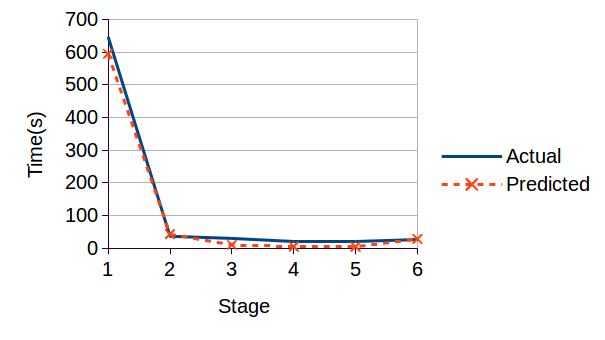
\includegraphics[width=3in]{pr20g_km_lr_wc.png}
\caption{Execution Time Prediction for PageRank Job Interfered with Other Three Jobs}
\label{pr20gkmlrwc}
\end{figure}
\begin{figure}[!t]
\centering
\captionsetup{justification=centering}
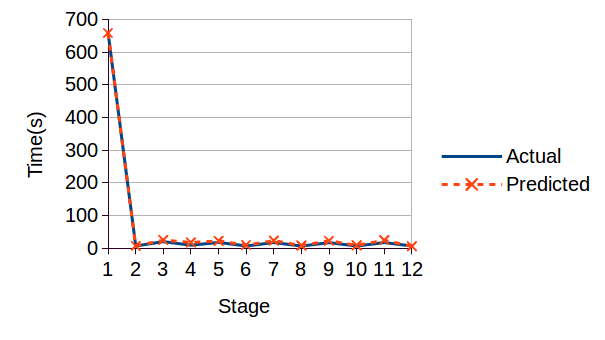
\includegraphics[width=3in]{km20g_pr_lr_wc.png}
\caption{Execution Time Prediction for K-Means Job Interfered with Other Three Jobs}
\label{km20gprlrwc}
\end{figure}
\begin{figure}[!t]
\centering
\captionsetup{justification=centering}
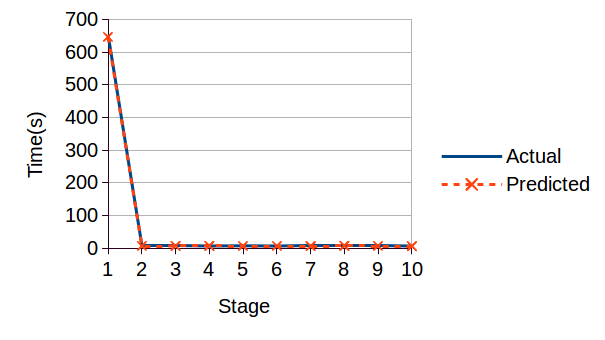
\includegraphics[width=3in]{lr20g_pr_km_wc.png}
\caption{Execution Time Prediction for Logistic Regression Job Interfered with Other Three Jobs}
\label{lr20gprkmwc}
\end{figure}
\begin{figure}[!t]
\centering
\captionsetup{justification=centering}
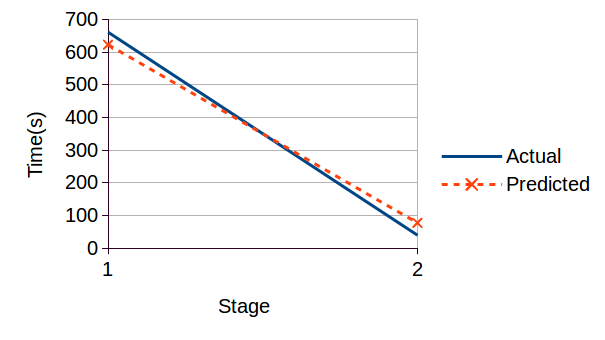
\includegraphics[width=3in]{wc20g_pr_km_lr.png}
\caption{Execution Time Prediction for WordCount Job Interfered with Other Three Jobs}
\label{wc20gprkmlr}
\end{figure}

}

\begin{table*}[!htb]
\renewcommand{\arraystretch}{1.3}
\caption{Execution Time Prediction for PageRank Job Interfered with Other Three Jobs}
\label{pr20gkmlrwc}
\centering
\begin{tabular}{l|r|r|r|r|r|r}
\hline
\bfseries StageNo & \bfseries 1 & \bfseries 2 & \bfseries 3 & \bfseries 4 & \bfseries 5 & \bfseries 6 \\
\hline \hline
Actual Time (s)
&646.4
&36.9
&30.4
&22.3
&21.8
&26.9 \\
\hline
Predicted Time (s) 
&594.3
&43.0
&10.6
&5.4
&5.0
&28.3 \\
\hline
\end{tabular}
\end{table*}

\begin{table*}[!htb]
\renewcommand{\arraystretch}{1.3}
\caption{Execution Time Prediction for K-Means Job Interfered with Other Three Jobs}
\label{km20gprlrwc}
\centering
\begin{tabular}{l|r|r|r|r|r|r|r|r|r|r|r|r}
\hline
\bfseries StageNo & \bfseries 1 & \bfseries 2 & \bfseries 3 & \bfseries 4 & \bfseries 5 & \bfseries 6 & \bfseries 7 & \bfseries 8 & \bfseries 9 & \bfseries 10 & \bfseries 11 & \bfseries 12\\
\hline \hline
Actual Time (s)
&657.4
&7.1
&20.6
&9.6
&18.1
&7.3
&17.8
&7.0
&17.4
&7.1
&17.7
&7.1 \\
\hline
Predicted Time (s) 
&657.4
&7.4
&25.2
&18.1
&22.9
&9.7
&23.6
&8.4
&23.2
&9.2
&24.8
&6.2 \\
\hline
\end{tabular}
\end{table*}

\begin{table*}[!htb]
\renewcommand{\arraystretch}{1.3}
\caption{Execution Time Prediction for Logistic Regression Job Interfered with Other Three Jobs}
\label{lr20gprkmwc}
\centering
\begin{tabular}{l|r|r|r|r|r|r|r|r|r|r}
\hline
\bfseries StageNo & \bfseries 1 & \bfseries 2 & \bfseries 3 & \bfseries 4 & \bfseries 5 & \bfseries 6 & \bfseries 7 & \bfseries 8 & \bfseries 9 & \bfseries 10 \\
\hline \hline
Actual Time (s)
&651.9
&7.3
&7.4
&7.1
&7.9
&7.1
&7.3
&7.2
&7.7
&7.1\\
\hline
Predicted Time (s) 
&646.0
&7.1
&7.2
&7.6
&6.6
&7.0
&6.5
&7.9
&6.9
&6.3\\
\hline
\end{tabular}
\end{table*}


\begin{table*}[!htb]
\renewcommand{\arraystretch}{1.3}
\caption{Execution Time Prediction for WordCount Job Interfered with Other Three Jobs}
\label{wc20gprkmlr}
\centering
\begin{tabular}{l|r|r}
\hline
\bfseries StageNo & \bfseries 1 & \bfseries 2 \\
\hline \hline
Actual Time (s)
&660.2
&40.2 \\
\hline
Predicted Time (s) 
&622.2
&77.8 \\
\hline
\end{tabular}
\end{table*}

\noindent
\begin{table*}[!t]
\renewcommand{\arraystretch}{1.3}
\caption{Prediction Accuracy for Two Different Jobs}
\label{table_twojobs}
\centering
\begin{tabular}{c|c|c|c}
\hline
\bfseries JobName & \bfseries Interfered Job & \bfseries First Stage & \bfseries Whole Job\\
\hline\hline
PR & KM & 0.91 & 0.79\\
& LR & 0.93 & 0.81\\
& WC & 0.99 & 0.85\\
\hline
KM & PR & 0.89 & 0.80\\
& LR & 0.80 & 0.73\\
& WC & 0.75 & 0.69\\
\hline
LR & PR & 0.97 & 0.97 \\
& KM & 0.73 & 0.77\\
& WC & 0.70 & 0.75\\ 
\hline
WC & PR & 0.96 & 0.87\\
& KM & 0.93 & 0.84\\
& LR & 0.96 & 0.88\\
\hline
\end{tabular}
\end{table*}


\begin{table*}[!htb]
\renewcommand{\arraystretch}{1.3}
\caption{Prediction Accuracy for Three Different Jobs}
\label{table_threejobs}
\centering
\begin{tabular}{c|c|c|c}
\hline
\bfseries JobName & \bfseries Interfered Jobs & \bfseries First Stage & \bfseries Whole Job\\
\hline\hline
PR & KM, LR & 0.96 & 0.87\\
& KM, WC & 0.99 & 0.90\\
& LR, WC & 0.99 & 0.90\\
\hline
KM & PR, LR & 0.84 & 0.79\\
& PR, WC & 0.92 & 0.87\\
& LR, WC & 0.83 & 0.80\\
\hline
LR & PR, KM & 0.84 & 0.85\\
& PR, WC & 0.87 & 0.88\\
& KM, WC & 0.83 & 0.84\\
\hline
WC & PR, LR & 0.93 & 0.87\\
& PR, KM & 0.93 & 0.87\\
& KM, LR & 0.94 & 0.89\\
\hline
\end{tabular}
\end{table*}


\begin{table*}[!htb]
\renewcommand{\arraystretch}{1.3}
\caption{Prediction Accuracy for Four Different Jobs}
\label{table_fourjobs}
\centering
\begin{tabular}{c|c|c|c}
\hline
\bfseries JobName & \bfseries Interfered Jobs & \bfseries First Stage & \bfseries Whole Job\\
\hline\hline
PR & KM, LR, WC & 0.92 & 0.86\\
\hline
KM & PR, LR, WC & 0.99 & 0.95\\
\hline
LR & PR, KM, WC & 0.99 & 0.99 \\
\hline
WC & PR, KM, LR & 0.95 & 0.90\\
\hline
\end{tabular}
\end{table*}


\subsection{Interference Among Multiple Jobs of Different Types Starting Simultaneously}
\noindent
In this section, we present the accuracy of prediction while modeling the interference among $n$ different jobs concurrently, where $n$ was varied from 2 to 4. For example, when $n$ = 2, we execute two different jobs concurrently. The prediction accuracy while running two different jobs in parallel is summarized in Table~\ref{table_twojobs}. As shown in the table, there are a total of 6 combinations to consider. As can be seen, prediction accuracy ranges between 97\% and 69\% for the whole job, and between 99\% and 70\% for the first stage, which incurs the bulk of the execution time. 

\noindent
For $n$=3, we execute three different jobs concurrently. The prediction accuracy while running three different jobs in parallel is summarized in Table~\ref{table_threejobs}. As shown in the table, there are a total of 4 combinations to consider. As can be seen, prediction accuracy ranges between 90\% and 79\% for the whole job, and between 99\% and 83\% for the first stage.

\noindent
Finally, for $n$=4, we execute four different jobs concurrently. The prediction accuracy while running four different jobs in parallel is summarized in Table~\ref{table_fourjobs}. As shown in the table, there was only one combination to consider. As can be seen, prediction accuracy ranges between 99\% and 86\% for the whole job, and between 99\% and 92\% for the first stage.
















\begin{table*}[!t]
\renewcommand{\arraystretch}{1.3}
\caption {Prediction Accuracy for Interference Among Different Jobs Starting at Different Times}
\label{table_differentjob_differentstarttime}
\centering
\begin{tabular}{c|c|c|c|c}
\hline

\bfseries Run & \bfseries JobName & \bfseries Starting Time(s) & \bfseries First Stage & \bfseries Whole Job\\
\hline\hline
Scenario - I & PR & 0 & 0.91 & 0.81\\
& KM & 38 & 0.99 & 0.94\\
& LR & 26 & 0.94 & 0.94 \\
& WC & 78 & 0.83 & 0.82\\
\hline
Scenario - II & PR & 91 & 0.90 & 0.82\\
& KM & 0 & 0.79 & 0.77\\
& LR & 48 & 0.87 & 0.88\\
& WC & 53 & 0.99 & 0.93\\
\hline
Scenario - III & PR & 20 & 0.99 & 0.90\\
& KM & 87 & 0.98 & 0.91\\
& LR & 0 & 0.84 & 0.85\\
& WC & 48 & 0.98 & 0.91\\
\hline
Scenario - IV & PR & 77 & 0.93 & 0.85\\
& KM & 25 & 0.72 & 0.71\\
& LR & 86 & 0.99 & 0.99 \\
& WC & 0 & 0.99 & 0.93\\
\hline
\end{tabular}
\end{table*} 



% Run B

\begin{table*}[!htb]
\renewcommand{\arraystretch}{1.3}
\caption{Execution Time Prediction for PageRank Job in Scenario - I}
\label{bpr}
\centering
\begin{tabular}{l|r|r|r|r|r|r}
\hline
\bfseries StageNo & \bfseries 1 & \bfseries 2 & \bfseries 3 & \bfseries 4 & \bfseries 5 & \bfseries 6 \\
\hline \hline
Actual Time (s)
&575.3
&36.4
&33.7
&24.1
&22.5
&55.8 \\
\hline
Predicted Time (s) 
&522.9
&43.0
&10.6
&5.4
&5.0
&28.3 \\
\hline
\end{tabular}
\end{table*}

\begin{table*}[!htb]
\renewcommand{\arraystretch}{1.3}
\caption{Execution Time Prediction for K-Means Job in Scenario - I}
\label{bkm}
\centering
\begin{tabular}{l|r|r|r|r|r|r|r|r|r|r|r|r}
\hline
\bfseries StageNo & \bfseries 1 & \bfseries 2 & \bfseries 3 & \bfseries 4 & \bfseries 5 & \bfseries 6 & \bfseries 7 & \bfseries 8 & \bfseries 9 & \bfseries 10 & \bfseries 11 & \bfseries 12\\
\hline \hline
Actual Time (s)
&611.8
&6.9
&21.0
&8.2
&18.0
&7.5
&17.6
&7.2
&17.5
&7.1
&17.3
&6.9 \\
\hline
Predicted Time (s) 
&610.7
&7.4
&25.2
&18.1
&22.9
&9.7
&23.6
&8.4
&23.2
&9.2
&24.8
&6.2 \\
\hline
\end{tabular}
\end{table*}

\begin{table*}[!htb]
\renewcommand{\arraystretch}{1.3}
\caption{Execution Time Prediction for Logistic Regression Job in Scenario - I}
\label{blr}
\centering
\begin{tabular}{l|r|r|r|r|r|r|r|r|r|r}
\hline
\bfseries StageNo & \bfseries 1 & \bfseries 2 & \bfseries 3 & \bfseries 4 & \bfseries 5 & \bfseries 6 & \bfseries 7 & \bfseries 8 & \bfseries 9 & \bfseries 10 \\
\hline \hline
Actual Time (s)
&576.8
&7.4
&7.3
&7.4
&7.2
&7.1
&7.8
&7.3
&7.2
&7.1 \\
\hline
Predicted Time (s) 
&617.1
&7.1
&7.2
&7.6
&6.6
&7.0
&6.5
&7.9
&6.9
&6.3
\\
\hline
\end{tabular}
\end{table*}


\begin{table*}[!htb]
\renewcommand{\arraystretch}{1.3}
\caption{Execution Time Prediction for WordCount Job in Scenario - I}
\label{bwc}
\centering
\begin{tabular}{l|r|r}
\hline
\bfseries StageNo & \bfseries 1 & \bfseries 2 \\
\hline \hline
Actual Time (s)
& 615.2
& 61.8 \\
\hline
Predicted Time (s) 
& 506.5
& 77.8 \\
\hline
\end{tabular}
\end{table*}



\subsection{Interference Among Multiple Jobs Starting at Different Times}
\label{newsection}
Finally, to test the prediction accuracy of our model where different jobs may arrive and start at different times, we use the four Apache Spark jobs and input data set as before, and start them randomly at different times. To ensure that each job will interfere with at least one other job while executing, we set the starting time for each job as $startingTime \in [minstagetime / 10, \\
minstagetime / 2]$, where $minstagetime$ represents the smallest execution time for the first stage among all the jobs. In our case, $minstagetime=190 sec$, causing the starting time for different jobs to be between 19 sec and 95 sec.

\noindent
Given the above range, for evaluation, we randomly pick one job and start at time 0, and then 
set the starting time for the remaining three jobs between 19 sec and 95 sec randomly. 
We considered four scenarios where the starting job is different in each scenario. The prediction accuracy for the whole job while running four different jobs in parallel starting at different times is summarized in Table~\ref{table_differentjob_differentstarttime}. As shown in the table, in our evaluation, prediction accuracy ranges between 99\% and 71\% for the whole job, and between 99\% and 72\% for the first stage. The predicted execution time and the actual execution time for PageRank, K-Means, Logistic Regression, and WordCount under Scenario - I are shown in Table~\ref{bpr}, Table~\ref{bkm}, Table~\ref{blr}, and Table~\ref{bwc} respectively. 




\subsection{Performance of Interference Aware Job Scheduling Algorithm}


To evaluate the performance of the job scheduling algorithm, we used the four Apache Spark jobs as before (e.g., PageRank (PR), K-Means (KM), Logistic Regression (LR) and WordCount (WC)). The order of job submission was varied in different experiments and the submission time was randomly chosen between 0 to 100 sec. The performance of our algorithm is compared against the default condition where each job is started immediately after submission. 

\noindent
In the first experiment, the four jobs were submitted in the order of PR, KM, LR, WC, and the input data size was set to 20GB for each of them. PR was submitted at $0s$, KM was submitted at $16s$, LR was submitted at $47s$, and WC was submitted at $94s$. As shown in Figure \ref{exp1}, the average execution time of individual jobs and total execution time (i.e., completion time of the last job minus the start time of the first job) were reduced by 47\% and 10\% respectively. 



\noindent
In the second experiment, the four jobs were submitted in the same order (PR, KM, LR, WC), but the input data size were set to 20GB for PR, 15GB for KM, 10GB for LR and 5GB for WC. PR was submitted at $0s$, KM was submitted at $59s$, LR was submitted at $88s$, and WC was submitted at $97s$. As shown in Figure \ref{exp2}, the average execution time of individual jobs and total execution time were reduced by 34\% and 13\% respectively. 

\noindent
In the third experiment, the four jobs were submitted in the order of KM, WC, PR, LR, and the input data size were set to 10GB for KM, 20GB for WC, 15GB for PR and 5GB for LR respectively. KM was submitted at $0s$, WC was submitted at $30s$, PR was submitted at $51s$, and LR was submitted at $71s$. As shown in Figure \ref{exp3}, the average execution time of individual jobs and total execution time were reduced by 26\% and 2\% respectively. 

\noindent
In the fourth experiment, the four jobs were submitted in the order of LR, WC, KM, PR, and the input data size were set to 15GB for LR, 10GB for WC, 20GB for KM and 15GB for PR respectively. LR was submitted at $0s$, WC was submitted at $8s$, KM was submitted at $53s$, and PR was submitted at $64s$. As shown in Figure \ref{exp4}, the average execution time of individual jobs and total execution time were reduced by 39\% and 8\% respectively. 

\noindent
In the fifth and last experiment, the four jobs were submitted in the order of WC, PR, LR, KM, and the input data size were set to 20GB for WC, 15GB for PR, 10GB for LR and 10GB for KM respectively. WC was submitted at $0s$, PR was submitted at $7s$, LR was submitted at $27s$, and KM was submitted at $71s$. As shown in Figure \ref{exp5}, the average execution time of individual jobs and total execution time were reduced by 40\% and 8\% respectively. 


\begin{figure}[!t]
\centering
\captionsetup{justification=centering}
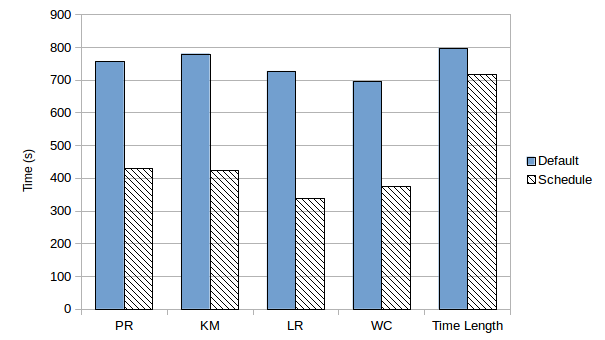
\includegraphics[width=3in]{exp1.png}
\caption{Result of Scheduling Experiment 1. Column Time length represents the total execution time (completion time of the last job minus the start time of the first job).}
\label{exp1}
\end{figure}

\begin{figure}[!t]
\centering
\captionsetup{justification=centering}
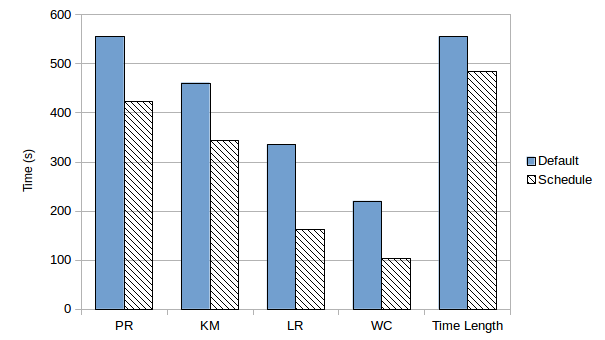
\includegraphics[width=3in]{exp2.png}
\caption{Result of Scheduling Experiment 2. Column Time length represents the total execution time (completion time of the last job minus the start time of the first job).}
\label{exp2}
\end{figure}

\begin{figure}[!t]
\centering
\captionsetup{justification=centering}
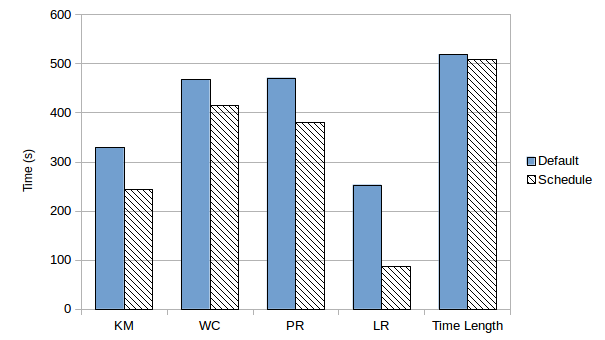
\includegraphics[width=3in]{exp3.png}
\caption{Result of Scheduling Experiment 3. Column Time length represents the total execution time (completion time of the last job minus the start time of the first job).}
\label{exp3}
\end{figure}



\begin{figure}[!t]
\centering
\captionsetup{justification=centering}
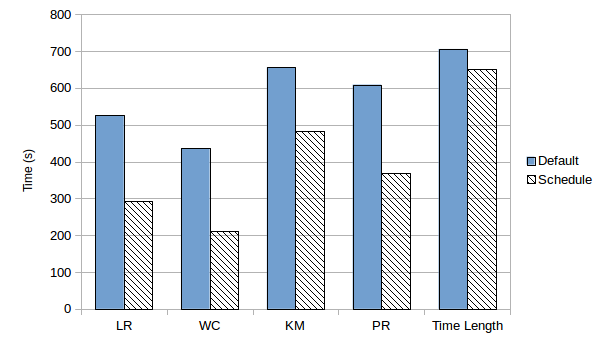
\includegraphics[width=3in]{exp4.png}
\caption{Result of Scheduling Experiment 4. Column Time length represents the total execution time (completion time of the last job minus the start time of the first job).}
\label{exp4}
\end{figure}





\begin{figure}[!t]
\centering
\captionsetup{justification=centering}
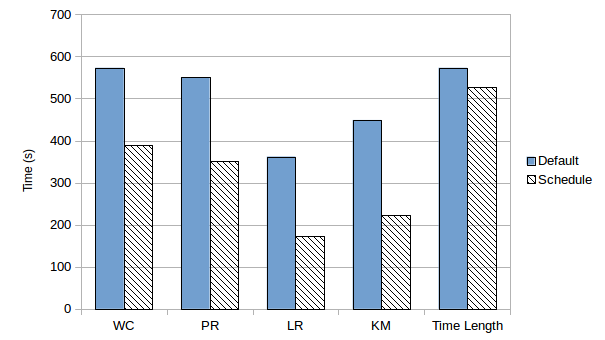
\includegraphics[width=3in]{exp5.png}
\caption{Result of Scheduling Experiment 5. Column Time length represents the total execution time (completion time of the last job minus the start time of the first job).}
\label{exp5}
\end{figure}


\section{Discussion}
\label{discussion}
While our model can predict performance degradation due to interference among multiple Apache Spark jobs with high accuracy, we do acknowledge several limitations of our current work as follows. First, our model assumes that the stages within a job are executed sequentially and does not consider the possibility of parallel execution, which will require extending our models. Second, the model was evaluated on 6 node cluster with 4 concurrent jobs, which is smaller compared to real-life clusters. Furthermore, the value $\beta_{n}$ depends on the number of concurrent jobs and needs to be calculated (once) as the number of concurrent jobs grows in a system. However, we strongly believe that our modeling framework will work well once the parameters are estimated for different cluster size and number of concurrent jobs in a system, which we plan to investigate in our future work. 







\section{Conclusion}
\label{conclusion}

\noindent
This paper presents a performance prediction framework for jobs running on Apache Spark platform. We establish models for predicting job performance by simulating the execution of actual job in a limited scale on real cluster. The prediction accuracy is evaluated for iterative and non-iterative algorithms. While the prediction accuracy is found to be high for execution time and memory, the I/O cost prediction varied for different applications. We strongly believe that our proposed approach can be used to predict job execution time with high-accuracy in real-life and will lead towards better resource allocation framework.  





\section{Acknowledgment} 
\noindent
This material is based upon work supported by the Air Force Office of Scientific Research award number FA9550-15-1-0184 under the DDDAS program. Any opinions, findings, and conclusions or recommendations expressed in this material are those of the authors and do not necessarily reflect the views of the funding agency.



%\bibliographystyle{IEEEtran}

% BibTeX users please use one of

%\bibliographystyle{spbasic}      % basic style, author-year citations

\bibliographystyle{spmpsci}      % mathematics and physical sciences
%\bibliographystyle{spphys}       % APS-like style for physics

\bibliography{paper}



\newpage
\newpage

\section{Appendix}
\label{appendix}

\begin{algorithm}[h]
\SetKwProg{Fn}{Function}{}{end}
\SetKwInput{KwIn}{Input}
\SetKwInput{KwOut}{Output}
\SetAlgoLined
\KwIn{List $JobProfiles$ listing Execution Information without Interference}
\KwOut{List $JobTime$ listing Execution Time with Interference}
\Fn {PredictJobExecution}{
Initialize List $Phases$, List $JobTime$\;
\For {all $job$ $\in$ $JobProfiles$ }{
$Phases$.add($job$.getStage(0)); //first stage\
}
\While{$Phases$.size $>$ 0}{ 
Initialize MinTime $\leftarrow$ MaxValue\;
\For {all $phase$ $\in$ $Phases$}{
r $\leftarrow$ $phase$.calculateSlowdownRatio($Phases$)\;
phaseTime $\leftarrow$ $phase$.getStageTime() $\times$ r\;
$phase$.setPhaseTime(phaseTime)\;
$phase$.setSlowdownRatio(r)\;
\If{phaseTime $<$ MinTime}{
MinTime $\leftarrow$ phaseTime\;
}
} 
\For {all $phase$ $\in$ $Phases$}{
\eIf{phase.getPhaseTime $=$ MinTime}{
StageTimeInterfere $\leftarrow$ MinTime $+$ $phase$.getPartialTime()\;
$JobTimes$.add($phase$ ,StageTimeInterfere)\;
$Phases$.remove($phase$)\;
\If{$JobProfiles$.hasNextStage($phase$)}{
nextStage $\leftarrow$ $JobProfiles$.nextStage($phase$)\;
$Phases$.add(nextStage)\; 
} 
}
{$phase$.setStageTime($phase$.getStageTime() $-$ $\frac{MinTime}{phase.getSlowdownRatio()}$)\;
$phase$.setPartialTime($phase$.getPartialTime $+$ MinTime)\;
}
}
}
}
\caption{Interference Estimation Algorithm}
\label{algo}
\end{algorithm}







\begin{algorithm}[h]
\SetKwProg{Fn}{Function}{}{end}
\SetKwInput{KwIn}{Input}
\SetKwInput{KwOut}{Output}
\SetAlgoLined{}
\KwIn{List $JobProfiles$ listing Execution Information without Interference}
\KwOut{List $JobsWaitingTime$ listing Job Waiting Time before scheduling}
\Fn {Scheduling}{
$JobProfiles \leftarrow $ CalculateExecutedTime($JobProfiles$) \;
$JobsWaitingTime \leftarrow$ FindWaitingTime($JobProfiles$) \;
}
\caption{Job Scheduling Algorithm}
\label{algoschedule}
\end{algorithm}


\begin{algorithm}[h]
\SetKwProg{Fn}{Function}{}{end}
\SetKwInput{KwIn}{Input}
\SetKwInput{KwOut}{Output}
\SetAlgoLined{}
\KwIn{List $JobProfiles$ listing Execution Information without Interference}
\KwOut{Remaining $JobProfiles$ after previous scheduling}
\Fn {CalculateExecutedTime}{
Initialize $SchInfo$, List $JobTimeLine$, Map $SlowdownRatios$, $ExeTime$\;
$SchInfo \leftarrow$ read($ScheduleFile$)\;
$LastExe \leftarrow SchInfo$.ExeTime()\;
$LastWait \leftarrow SchInfo$.WaitTime()\;
JobsUpdate($JobProfiles$,$LastExe$,$LastWait$)\;
$interval \leftarrow$ CurrentTime $- SchInfo$.SubTime()\;
\For {all $job \in JobProfiles$}{
$JobTimeLine$.add($job$.getStage(0).getBegin())\;
$JobTimeLine$.add($job$.getStage(0).getEnd())\;
$R \leftarrow job$.getStage(0).calculateSlowdownRatios()\;
$SlowdownRatios$.put($job$,$R$)\;
}
Initialize List $ParallelJobs$\;
\For {all $Timepoint \in JobTimeLine$}{
\If{ $Timepoint > interval$}{
%$isFinish \leftarrow$ True\;
$Timepoint$.setValue($interval$)\;
}
$gap \leftarrow Timepoint- LastTimepoint$\;
$job \leftarrow Timepoint$.getJob()\;
\For{all $job \in ParallelJobs$}{
$p \leftarrow ParallelJobs$.size() $-$ 1\;
$ExeTime$.put($job$,$ExeTime$.get($job$) $+ gap \times SlowdownRatios$.get($job$).get($p$))\;
}
\eIf{$Timepoint$.isBegin()}{
$ParallelJobs$.add($job$)\;
}{
$lefttime \leftarrow job$.getDuration() $- job$.getStage(0).getDuration()\;
\eIf{$lefttime > interval - Timepoint$}{
$ExeTime$.put($job$,$ExeTime$.get($job$) $+ interval - Timepoint$.)\;
}{
$ExeTime$.put($job$,$ExeTime$.get($job$) $+ lefttime$)\;
}
$ParallelJobs$.remove($job$)\;
}
$LastTimepoint \leftarrow Timepoint$\; 
%\If{$isFinish$}{
%break\;}
}
JobsUpdate($JobProfiles$,$LastWait$,0)\;
JobsUpdate($JobProfiles$,$ExeTime$,0)\;
}
\caption{Calculate Executed Time}
\label{algoexe}
\end{algorithm}









\begin{algorithm}[h]
\SetKwProg{Fn}{Function}{}{end}
\SetKwInput{KwIn}{Input}
\SetKwInput{KwOut}{Output}
\SetAlgoLined{}
\KwIn{List $JobProfiles, ExeTime, WaitTime$}
\KwOut{Updated List $JobProfiles$}
\Fn {JobsUpdate}{
\For {all $job \in JobProfiles$ }{
\If{$ExeTime$.get($job$) $>$ 0}{
$job$.minus($ExeTime$.get($job$))\;
}
\If{$WaitTime$.get($job$) $>$ 0}{
$job$.addStart($WaitTime$.get($job$))\;
}
}
}
\caption{JobProfile Update}
\label{algoupdate}
\end{algorithm}


\begin{algorithm}[h]
\SetKwProg{Fn}{Function}{}{end}
\SetKwInput{KwIn}{Input}
\SetKwInput{KwOut}{Output}
\SetAlgoLined{}
\KwIn{List $JobProfiles$ listing Execution Information without Interference}
\KwOut{List $JobsWaitingTime$ listing Job Waiting Time before scheduling}
\Fn {FindWaitingTime}{
Initialize $WaitN$, $minTime$, Map $JobsWait$, List $JobsWaitingTime$\;
$JobTime$ $\leftarrow$ $PredictJobExecution$($JobProfiles$)\;
\For {all $job \in JobProfiles$ }{
$waitTimeMax \leftarrow JobTime$.getMax() $- job$.getDuration()\;
\For{$i \gets 0$ to $WaitN$}{
$Jobwait$.add($\frac{i}{WaitN}\times waitTimeMax$) \;
}
$JobsWait$.put($job$,$Jobwait$)\;
}
\For{ $Jobswait \in \prod_{i=1}^{N} JobsWait.get(i) $}{
JobsUpdate($JobProfiles$,0,$Jobswait$)\;
$JobTime$ $\leftarrow$ $PredictJobExecution$($JobProfiles$)\;
\If{$JobTime$.getMax() $< minTime$}{
$minTime \leftarrow JobTime$.getMax() \;
$JobsWaitingTime \leftarrow Jobswait$\;
}

}
}
\caption{Find Waiting Time}
\label{algofind}
\end{algorithm}









\end{document}


